\begin{ex}
(UF – MG) Observe o diagrama:

\begin{center}    
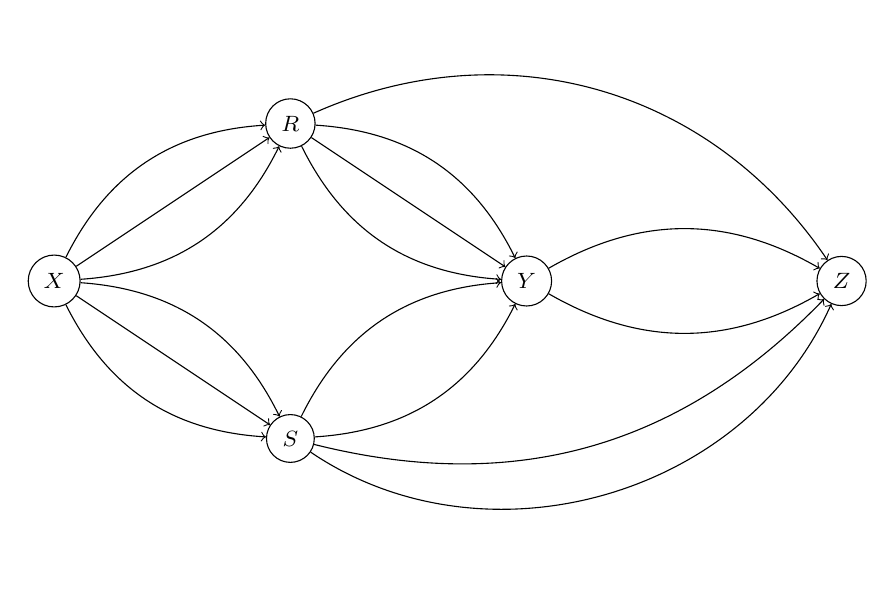
\begin{tikzpicture}
\tikzset{
vertex/.style={circle,draw,minimum size=1em},
edge/.style={->,> = latex'},
font={\fontsize{8pt}{10}\selectfont}
}


\node[vertex] (X) at (-5,0) {$X$};
\node[vertex] (Y) at (1,0) {$Y$};
\node[vertex] (Z) at (5,0) {$Z$};
\node[vertex] (R) at (-2,2) {$R$};
\node[vertex] (S) at (-2,-2) {$S$};


\path[->]
 (R) edge (Y)
 (R) edge[bend left=30] (Y)                              
 (R) edge[bend right=30] (Y)                               
 (R) edge[bend left=40] (Z)                              
 
 (Y) edge[bend left=30] (Z)
 (Y) edge[bend right=30] (Z)
 
 (S) edge[bend left=30] (Y)
 (S) edge[bend right=30] (Y)
 (S) edge[bend right=30] (Z)
 (S) edge[bend right=50] (Z)

 (X) edge[bend left=30] (R)                              
 (X) edge[bend right=30] (R)                              
 (X) edge (R)                              

 (X) edge[bend left=30] (S)                              
 (X) edge[bend right=30] (S)                              
 (X) edge (S)                              
;
\end{tikzpicture}
\end{center}

Qual é o número de ligações distintas entre X e Z?
 \begin{sol}
   \phantom{A} \\
   ligações entre X e Z $\rightarrow $ X R Z ou X S Z ou X R Y Z ou X Y Z ou X S Y Z \\
   $3\cdot1 +3\cdot2 + 3\cdot3\cdot2+1\cdot2+3\cdot2\cdot2=41$
 \end{sol}
\end{ex}